% snapshot_v1_report.tex
% Literature Snapshot v1 — La(Fe,Si)13 Magnetocaloric Data Layer
% I. Radulov · 7 November 2026
% Compile: pdflatex snapshot_v1_report.tex  (twice for cross-refs)

\documentclass[11pt,a4paper]{article}

\usepackage[T1]{fontenc}
\usepackage[utf8]{inputenc}
\usepackage{lmodern}
\usepackage[margin=25mm]{geometry}
\usepackage{booktabs}
\usepackage{array}
\usepackage{longtable}
\usepackage{xcolor}
\usepackage{listings}
\usepackage{hyperref}
\usepackage{microtype}
\usepackage{parskip}
\usepackage{caption}
\usepackage{tikz}
\usetikzlibrary{positioning, shapes.geometric, arrows.meta, fit, backgrounds, calc}

% ── colour palette ──────────────────────────────────────────────────────────
\definecolor{tblue}{HTML}{1A5276}
\definecolor{tgreen}{HTML}{1E8449}
\definecolor{tgray}{HTML}{5D6D7E}
\definecolor{tlightblue}{HTML}{D6EAF8}
\definecolor{tlightgreen}{HTML}{D5F5E3}
\definecolor{tlightgray}{HTML}{F2F3F4}
\definecolor{codebg}{HTML}{F8F9FA}
\definecolor{commentgray}{HTML}{7F8C8D}

% ── listings style ──────────────────────────────────────────────────────────
\lstdefinestyle{terminal}{
  backgroundcolor=\color{codebg},
  basicstyle=\ttfamily\footnotesize,
  breaklines=true,
  breakatwhitespace=false,
  frame=single,
  framesep=4pt,
  rulecolor=\color{tgray},
  xleftmargin=6pt,
  xrightmargin=6pt,
  aboveskip=8pt,
  belowskip=4pt,
  keepspaces=true,
  columns=flexible,
  showstringspaces=false,
  commentstyle=\color{commentgray}\itshape,
}
\lstdefinestyle{sql}{
  backgroundcolor=\color{codebg},
  basicstyle=\ttfamily\footnotesize,
  breaklines=true,
  frame=single,
  framesep=4pt,
  rulecolor=\color{tgray},
  xleftmargin=6pt,
  xrightmargin=6pt,
  aboveskip=8pt,
  belowskip=4pt,
  keepspaces=true,
  columns=flexible,
  morekeywords={SELECT,FROM,WHERE,GROUP,BY,COUNT,SET,search_path,ORDER,AS,
                CONSTRAINT,FOREIGN,KEY,REFERENCES,ON,DELETE,CASCADE,
                PRIMARY,UNIQUE,NOT,NULL,DEFAULT,CREATE,TABLE,INDEX},
  keywordstyle=\color{tblue}\bfseries,
  commentstyle=\color{commentgray}\itshape,
  morecomment=[l]{--},
}

\hypersetup{colorlinks=true, linkcolor=tblue, urlcolor=tblue, citecolor=tblue}

% ── TikZ styles ─────────────────────────────────────────────────────────────
\tikzset{
  entity/.style={
    rectangle, draw=tblue, fill=tlightblue,
    rounded corners=3pt,
    text width=#1, align=left,
    font=\ttfamily\footnotesize,
    inner sep=6pt,
  },
  entity/.default=52mm,
  entitytitle/.style={
    font=\ttfamily\small\bfseries\color{tblue},
  },
  fk/.style={
    ->, >=Stealth, thick, draw=tblue,
  },
  fkdash/.style={
    ->, >=Stealth, thick, draw=tgray, dashed,
  },
  pipenode/.style={
    rectangle, draw=tgreen, fill=tlightgreen,
    rounded corners=4pt,
    text width=36mm, align=center,
    font=\small,
    inner sep=7pt, minimum height=10mm,
  },
  pipearrow/.style={
    ->, >=Stealth, thick, draw=tgreen,
  },
  annot/.style={
    font=\scriptsize\itshape\color{tgray},
    align=center,
  },
}

% ── helpers ─────────────────────────────────────────────────────────────────
\newcommand{\col}[2]{\textbf{#1} \textcolor{tgray}{\textit{#2}}}
\newcommand{\pk}[1]{\textcolor{tblue}{\underline{\textbf{#1}}}}
\newcommand{\fkcol}[1]{\textcolor{tgreen}{\textbf{#1}}}
\newcommand{\snap}{\textit{Snapshot~v1}}

% ────────────────────────────────────────────────────────────────────────────
\begin{document}

\begin{center}
  {\LARGE\bfseries Literature Snapshot v1}\\[4pt]
  {\large La(Fe,Si)$_{13}$ Magnetocaloric Data Layer}\\[8pt]
  {\large I.~Radulov} \quad·\quad 7~November~2026\\[4pt]
  {\small\color{tgray}
    Repository: \texttt{iliya-radulov/my\_db\_project} \quad
    Branch: \texttt{main} \quad
    Database: \texttt{alloy\_lab} @ \texttt{192.168.178.10}}
\end{center}

\vspace{2mm}\hrule\vspace{6mm}

% ────────────────────────────────────────────────────────────────────────────
\section{Purpose of this document}

This report records the state of the La(Fe,Si)$_{13}$ literature database on
7~November~2026 (\snap).  It serves three purposes:
\begin{itemize}
  \item a reproducibility anchor: anyone can re-run the commands in
        Section~\ref{sec:checks} and obtain identical counts;
  \item a methods section for the Stage~4 Track~B paper
        (the database design described in Section~\ref{sec:schema} is
        the first contribution of that paper);
  \item a decision log: data-source licences and the train/test
        separation are recorded in Section~\ref{sec:sources}.
\end{itemize}

% ────────────────────────────────────────────────────────────────────────────
\section{Snapshot numbers}

\begin{center}
\begin{tabular}{lrrl}
  \toprule
  Item & Count & & Note \\
  \midrule
  Records (\texttt{mce\_literature\_records}) & 1\,113 & & from 221 papers \\
  Measurement points (\texttt{mce\_literature\_points}) & 1\,539 & &
        1\,386 $|\Delta s_T|$ + 153 $|\Delta T_\mathrm{ad}|$ \\
  Distinct composition keys & 660 & &
        129 keys appear in $>$1 paper (duplicates kept) \\
  Lab samples with exact literature match & 7 & &
        matched to 180 records \\
  Sources currently loaded & 1 & & \texttt{nims\_lafesi\_1\_13} \\
  \bottomrule
\end{tabular}
\captionof{table}{\snap{} counts, confirmed 7~Nov~2026.}
\end{center}

% ────────────────────────────────────────────────────────────────────────────
\section{Database schema}
\label{sec:schema}

\subsection{Overview}

The literature data live in two tables (\texttt{mce\_literature\_records}
and \texttt{mce\_literature\_points}) that are linked by a foreign key.
A bridge table (\texttt{sample\_composition\_keys}) connects the literature
records to the lab samples via a normalised composition key.
Figure~\ref{fig:er} shows the entity–relationship diagram.

\subsection{Composition key}

The composition key is the central join field.  It is computed from the
element amounts as follows:
\begin{enumerate}
  \item Metal elements (La, Fe, Si, Mn, Cr, Ni, Co, \ldots) are
        normalised so their atom-percent sum equals 100\,at.\%.
  \item Interstitial elements (H, C, N, B) are stored separately,
        appended after a \texttt{+} sign.
  \item All amounts are rounded to 0.1\,at.\% resolution.
\end{enumerate}
Example: \texttt{Fe81.4-La7.1-Si11.4+H3.6}.
Two records are an exact match if and only if their composition keys are
identical.  This rule is intentionally strict: a composition reported as
La$_1$Fe$_{11.4}$Si$_{1.6}$ in one paper and La$_1$Fe$_{11.3}$Si$_{1.7}$
in another yields two distinct keys and is kept as two separate records.

\subsection{Entity--relationship diagram}

\begin{figure}[h]
\centering
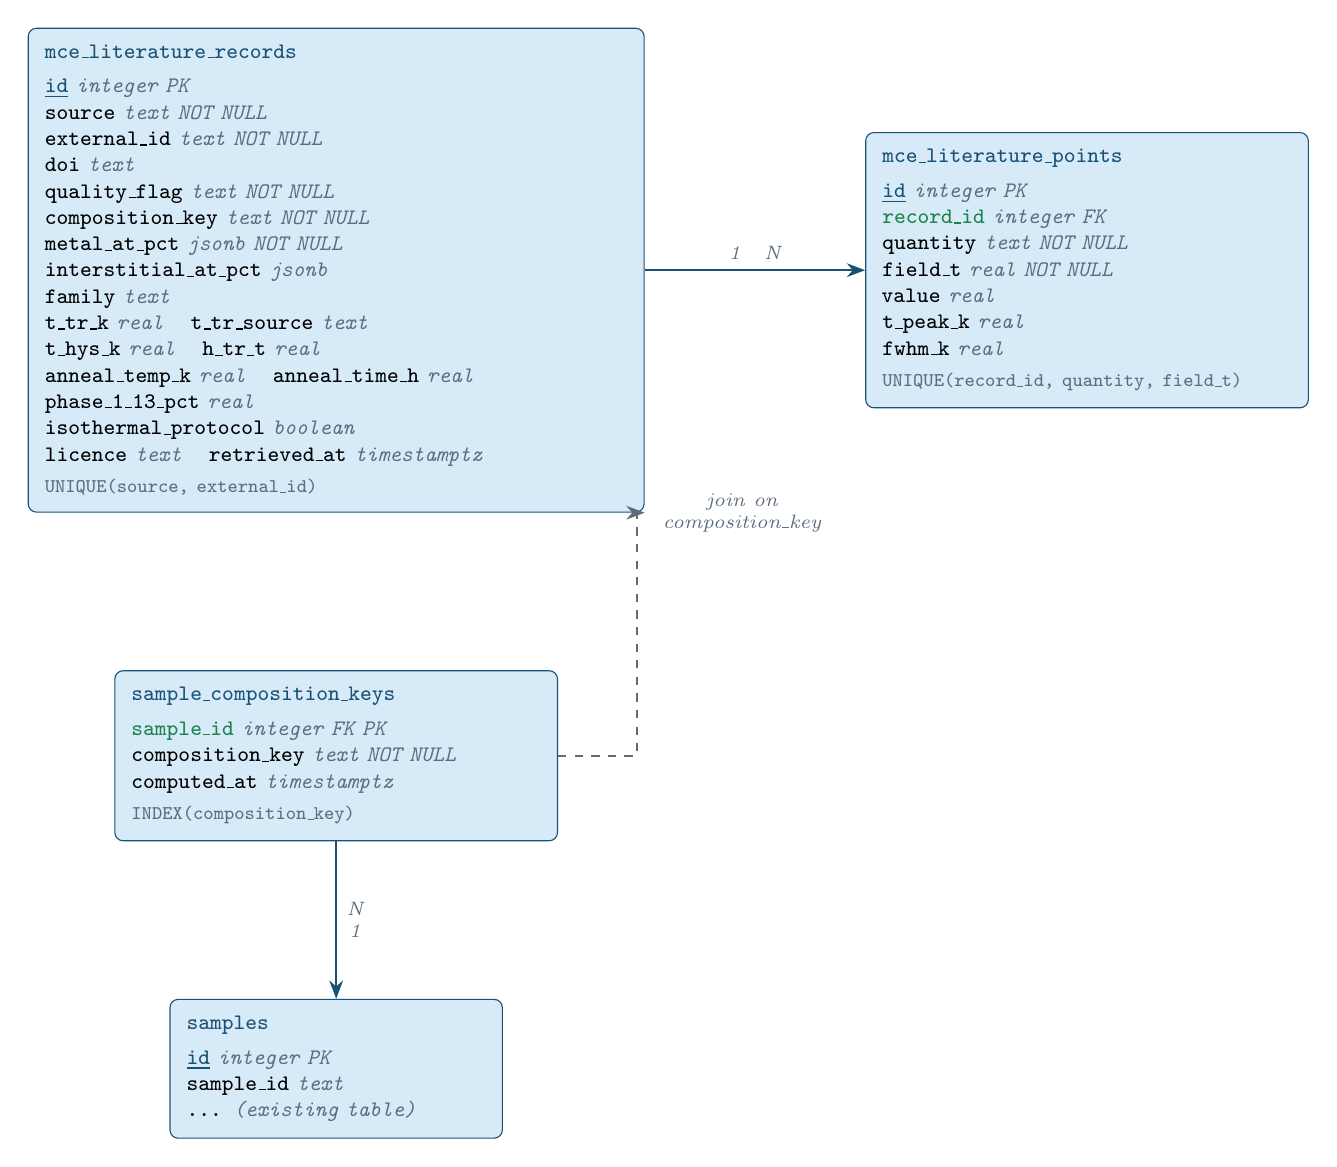
\begin{tikzpicture}[node distance=14mm and 20mm]

%% ── mce_literature_records ──────────────────────────────────────────────
\node[entity=74mm] (rec) {%
  \textbf{\color{tblue}mce\_literature\_records}\\[3pt]
  \pk{id} \textcolor{tgray}{\textit{integer PK}}\\
  \col{source}{text NOT NULL}\\
  \col{external\_id}{text NOT NULL}\\
  \col{doi}{text}\\
  \col{quality\_flag}{text NOT NULL}\\
  \col{composition\_key}{text NOT NULL}\\
  \col{metal\_at\_pct}{jsonb NOT NULL}\\
  \col{interstitial\_at\_pct}{jsonb}\\
  \col{family}{text}\\
  \col{t\_tr\_k}{real}\quad\col{t\_tr\_source}{text}\\
  \col{t\_hys\_k}{real}\quad\col{h\_tr\_t}{real}\\
  \col{anneal\_temp\_k}{real}\quad\col{anneal\_time\_h}{real}\\
  \col{phase\_1\_13\_pct}{real}\\
  \col{isothermal\_protocol}{boolean}\\
  \col{licence}{text}\quad\col{retrieved\_at}{timestamptz}\\[2pt]
  \textcolor{tgray}{\scriptsize UNIQUE(source, external\_id)}
};

%% ── mce_literature_points ───────────────────────────────────────────────
\node[entity=52mm, right=28mm of rec] (pts) {%
  \textbf{\color{tblue}mce\_literature\_points}\\[3pt]
  \pk{id} \textcolor{tgray}{\textit{integer PK}}\\
  \fkcol{record\_id} \textcolor{tgray}{\textit{integer FK}}\\
  \col{quantity}{text NOT NULL}\\
  \col{field\_t}{real NOT NULL}\\
  \col{value}{real}\\
  \col{t\_peak\_k}{real}\\
  \col{fwhm\_k}{real}\\[2pt]
  \textcolor{tgray}{\scriptsize UNIQUE(record\_id, quantity, field\_t)}
};

%% ── sample_composition_keys ─────────────────────────────────────────────
\node[entity=52mm, below=20mm of rec] (sck) {%
  \textbf{\color{tblue}sample\_composition\_keys}\\[3pt]
  \fkcol{sample\_id} \textcolor{tgray}{\textit{integer FK PK}}\\
  \col{composition\_key}{text NOT NULL}\\
  \col{computed\_at}{timestamptz}\\[2pt]
  \textcolor{tgray}{\scriptsize INDEX(composition\_key)}
};

%% ── samples (stub) ──────────────────────────────────────────────────────
\node[entity=38mm, below=20mm of sck] (smp) {%
  \textbf{\color{tblue}samples}\\[3pt]
  \pk{id} \textcolor{tgray}{\textit{integer PK}}\\
  \col{sample\_id}{text}\\
  \col{\ldots}{(existing table)}
};

%% ── arrows ──────────────────────────────────────────────────────────────
% record → points  (1:N)
\draw[fk] (rec.east) -- node[above, annot]{1\quad N} (pts.west);

% sample_composition_keys → samples  (N:1)
\draw[fk] (sck.south) -- node[right, annot]{N\\1} (smp.north);

% join via composition_key (dashed)
\draw[fkdash]
  (sck.east) --++(10mm,0) |- node[right, annot, xshift=2mm]{join on\\composition\_key}
  (rec.south east);

\end{tikzpicture}
\caption{Entity--relationship diagram of the literature data layer.
  Solid arrows are foreign-key constraints; the dashed arrow is a
  logical join on \texttt{composition\_key} (no FK constraint — a
  literature record may have no matching lab sample and vice versa).
  Primary keys are \underline{underlined}; foreign keys are in
  \textcolor{tgreen}{green}.}
\label{fig:er}
\end{figure}

% ────────────────────────────────────────────────────────────────────────────
\section{Import pipeline}
\label{sec:pipeline}

Figure~\ref{fig:pipeline} shows the full flow from the raw NIMS file to
the verified database state.

\begin{figure}[h]
\centering
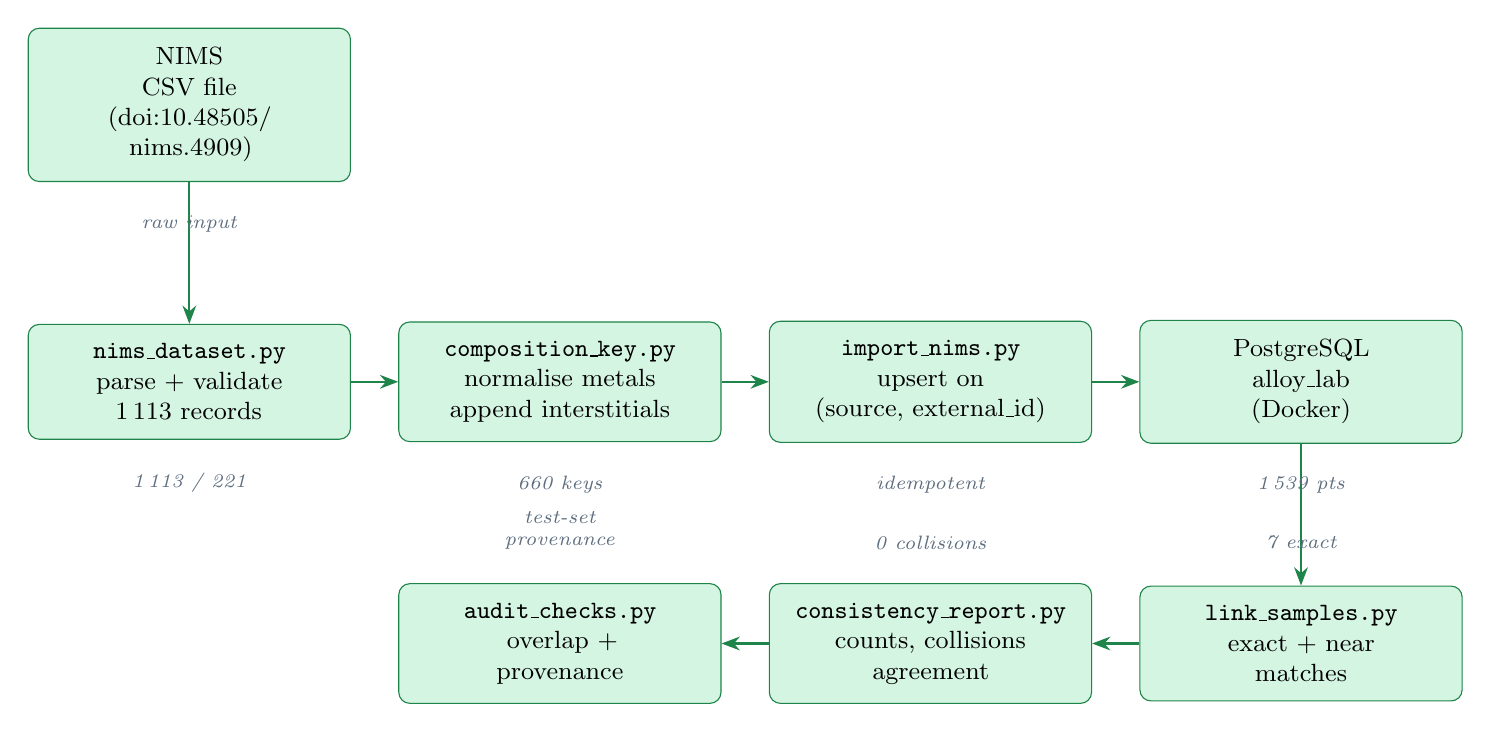
\begin{tikzpicture}[node distance=2mm and 6mm]

\node[pipenode] (nims) {NIMS\\CSV file\\(doi:10.48505/\\nims.4909)};

\node[pipenode, below=18mm of nims] (parse) {\texttt{nims\_dataset.py}\\parse + validate\\1\,113 records};

\node[pipenode, right=of parse] (key) {\texttt{composition\_key.py}\\normalise metals\\append interstitials};

\node[pipenode, right=of key] (upsert) {\texttt{import\_nims.py}\\upsert on\\(source, external\_id)};

\node[pipenode, right=of upsert] (db) {PostgreSQL\\alloy\_lab\\(Docker)};

\node[pipenode, below=18mm of db] (link) {\texttt{link\_samples.py}\\exact + near\\matches};

\node[pipenode, left=of link] (cons) {\texttt{consistency\_report.py}\\counts, collisions\\agreement};

\node[pipenode, left=of cons] (audit) {\texttt{audit\_checks.py}\\overlap +\\provenance};

\draw[pipearrow] (nims) -- (parse);
\draw[pipearrow] (parse) -- (key);
\draw[pipearrow] (key) -- (upsert);
\draw[pipearrow] (upsert) -- (db);
\draw[pipearrow] (db) -- (link);
\draw[pipearrow] (link) -- (cons);
\draw[pipearrow] (cons) -- (audit);

\node[annot, below=3mm of nims]  {raw input};
\node[annot, below=3mm of parse] {1\,113 / 221};
\node[annot, below=3mm of key]   {660 keys};
\node[annot, below=3mm of upsert]{idempotent};
\node[annot, below=3mm of db]    {1\,539 pts};
\node[annot, above=3mm of link]  {7 exact};
\node[annot, above=3mm of cons]  {0 collisions};
\node[annot, above=3mm of audit] {test-set\\provenance};

\end{tikzpicture}
\caption{Import and verification pipeline for \snap{}.
  Every step is re-runnable; the upsert is idempotent.}
\label{fig:pipeline}
\end{figure}

\newpage
% ────────────────────────────────────────────────────────────────────────────
\section{Verification checks}
\label{sec:checks}

All four checks were run on 7~November~2026 from the desktop machine
(\texttt{192.168.178.47}) against the server (\texttt{192.168.178.10}).\\

The working directory was
\texttt{\textasciitilde/Documents/github/active/my\_db\_project/stage\_four/mce\_nims/}.

\subsection{Record and point counts}

\begin{lstlisting}[style=terminal, caption={Database record counts.}]
$ ssh r@192.168.178.10 "docker exec alloy-postgres psql -U postgres \
    -d alloy_lab -c 'SELECT source, COUNT(*) as records \
    FROM alloy_lab.mce_literature_records GROUP BY source;'"

      source      | records
------------------+---------
 nims_lafesi_1_13 |    1113
(1 row)

$ ssh r@192.168.178.10 "docker exec alloy-postgres psql -U postgres \
    -d alloy_lab -c 'SELECT COUNT(*) as points \
    FROM alloy_lab.mce_literature_points;'"

 points
--------
   1539
(1 row)
\end{lstlisting}

\newpage

\subsection{Import idempotency (\texttt{import\_nims.py --dry-run} and live run)}

\begin{lstlisting}[style=terminal, caption={Dry-run and live import confirming idempotency.}]
$ python import_nims.py --dry-run
1113 records from 221 papers
  T_tr: {'reported': 835, 'dS_peak': 98, 'dS_dTad_mean': 26,
         'dTad_peak': 21}, missing 134
  dS_max points: 1386, dT_ad_max points: 153
  composition keys: 660 distinct; 129 keys appear in more than one paper
  quality_flag: 'experimental_literature' for all 1113 records
  dS: list lengths differ from the field list, values left empty:
      [(530, 'T_at_dS_max_K'), (531, 'T_at_dS_max_K')]

$ python import_nims.py
[... same summary lines ...]
Connected to database: alloy_lab
Imported 1113 records and 1539 points (source 'nims_lafesi_1_13')
\end{lstlisting}

The two list-length warnings on rows 530 and 531 are pre-existing entries
in the NIMS source file (the temperature list has one fewer entry than the
value list); the affected \texttt{T\_at\_dS\_max\_K} cells are left empty.
This is not an import error.

\subsection{Sample linking (\texttt{link\_samples.py})}

\begin{lstlisting}[style=terminal, caption={Sample--literature linking output (abbreviated).}]
$ python link_samples.py
Connected to database: alloy_lab
73 samples: 44 keyed, 29 skipped
  skipped New_test_sample: not element symbols: ['placeholder']
  [... 28 further placeholder entries omitted ...]

Exact matches: 7 samples
  La1Fe113Si17-20260713-001  Fe80.7-La7.1-Si12.1   4 records from 4 papers
  La1Fe113Si17-20260713-002  Fe80.7-La7.1-Si12.1   4 records from 4 papers
  La1Fe114Si16-20260708-001  Fe81.4-La7.1-Si11.4  29 records from 21 papers
  La1Fe115Si15-20260708-001  Fe82.1-La7.1-Si10.7  40 records from 32 papers
  La1Fe115Si15-20260711-002  Fe82.1-La7.1-Si10.7  40 records from 32 papers
  La1Fe116Si14-20260708-001  Fe82.9-La7.1-Si10.0  50 records from 36 papers
  La1Fe118Si12-20260709-001  Fe84.3-La7.1-Si8.6   13 records from 8 papers

Near matches (every element within 0.5 at.%, excluding exact matches):
  La1Fe116Si14-20260708-001  Fe82.9-La7.1-Si10.0
    22 records; closest: nims_lafesi_1_13:174 (0.03 at.%)
  [...]
  La103Fe115Mn01Si14-20260902-001  Fe82.0-La7.3-Mn0.7-Si10.0
    3 records; closest: nims_lafesi_1_13:34 (0.20 at.%)
\end{lstlisting}

The 29 skipped samples all have \texttt{['placeholder']} as their
composition entry — these are test or incomplete entries in the
\texttt{samples} table and are expected to be absent from the matching.

\newpage

\subsection{Consistency report (\texttt{consistency\_report.py})}

\begin{lstlisting}[style=terminal, caption={Consistency report output.}]
$ python consistency_report.py
Connected to database: alloy_lab

Per source
  source            quality_flag             records  papers  keys  with_t_tr
  nims_lafesi_1_13  experimental_literature  1113     221     660   979

Points per source
  source            quantity   points  records
  nims_lafesi_1_13  dS_max     1386    820
  nims_lafesi_1_13  dT_ad_max  153     128

New compositions (keys found in only this source)
  source            keys_only_here
  nims_lafesi_1_13  660

Collisions between sources
  keys_in_several_sources  papers_in_several_sources
  0                        0

Agreement where two sources have the same paper and composition key
  (none)

Own samples with exact matches
  source            quality_flag             samples  matched_records
  nims_lafesi_1_13  experimental_literature  7        180
\end{lstlisting}

Zero collisions are expected at \snap{}: the NIMS dataset is the only
source loaded.  The collision and agreement metrics become meaningful in
Snapshot~v2 once MCEdatabase and the Kelly \& Cole datasets are imported.

\subsection{Bracket-composition audit (section~4b of \texttt{SERVER\_SETUP.md})}

This check identifies samples whose composition was entered with brackets
or signs in the formula field, which an earlier version of the parser
would have silently mis-parsed.

\begin{lstlisting}[style=sql, caption={SQL audit for bracket-formula entries.}]
SET search_path TO alloy_lab;
SELECT sample_id, created_at, notes FROM samples
WHERE notes ~ 'Desktop App: .*[()\[\]{}+\-,;/]'
ORDER BY created_at;
\end{lstlisting}

\begin{lstlisting}[style=terminal, caption={Bracket audit result.}]
           sample_id            |         created_at         | notes
--------------------------------+----------------------------+---------------
 Fe195Co005P09Si01-20260714-001 | 2026-07-14 09:51:20.501258 |
   Added via Desktop App: pre-alloy Fe2P (10g)
   + raw Fe1.95Co0.05P0.9Si0.1 (at%)
(1 row)
\end{lstlisting}

One hit: a pre-alloy entry for a Fe$_2$P-family compound (not
La(Fe,Si)$_{13}$).  The note format \texttt{pre-alloy \ldots\ (g) + raw
\ldots\ (at\%)} is the expected pre-alloy pattern documented in
\texttt{SERVER\_SETUP.md} and requires no action.

% ────────────────────────────────────────────────────────────────────────────
\section{Data sources and licences}
\label{sec:sources}

\begin{center}
\begin{tabular}{p{42mm}p{18mm}p{22mm}p{55mm}}
  \toprule
  Source & Status & Licence & Notes \\
  \midrule
  NIMS La(Fe,Si)$_{13}$ \newline doi:10.48505/nims.4909
    & \textcolor{tgreen}{\bfseries Imported}
    & CC BY 4.0
    & 1\,113 records / 221 papers; file not committed to git \\[4pt]
  MCEdatabase \newline github.com/RunqingYang1996 \newline /MCEdatabase
    & \textcolor{tgreen}{\bfseries Permission confirmed}
    & Author email \newline (Bolin Lau / \newline Xuchao, 2 Nov 2026)
    & Reuse with citation of Yuan et al.; $\approx$202 records,
      50 La(Fe,Si)$_{13}$ papers not in NIMS; not yet imported \\[4pt]
  Kelly \& Cole 2025 \newline figshare 29559686
    & \textcolor{tgray}{Not yet imported}
    & CC BY 4.0 \newline (figshare)
    & $\approx$100 records; direct contact not replied;
      figshare licence sufficient to proceed \\[4pt]
  Court \& Cole 2018 \newline figshare c.3954418
    & \textcolor{tgray}{Not yet imported}
    & CC BY 4.0 \newline (figshare)
    & $\approx$80 records; same as above \\[4pt]
  Dr.\ H.\ Ucar — Heusler dataset
    & \textcolor{tgreen}{\bfseries Received}
    & Personal comm.
    & $\approx$500 Heusler records (Victorino 2018/19 + new);
      \textbf{future scope only} — not La(Fe,Si)$_{13}$ \\
  \bottomrule
\end{tabular}
\captionof{table}{Data sources at \snap{}. The NIMS file is kept only on
  the server and is not committed to the repository (CC~BY~4.0 requires
  attribution but does not restrict private hosting).}
\end{center}

\subsection*{Train / test separation (hard constraint)}

The Moreno-Ram\'{i}rez Ni and Cr papers are the held-out test set and
are \textbf{never} used for training.  This constraint is enforced in
\texttt{evaluate.py} and must not be changed without a new snapshot
document.

\subsection*{Training data decision}

Adding MCEdatabase, Kelly \& Cole, and Court \& Cole to the NIMS training
data showed no improvement in LOFO cross-validation MAE (pre-registered
criterion, evaluated $\approx$4~November~2026).  The decision: \textbf{train
on NIMS only}.  The additional sources are retained as provenance records
and may be used as independent held-out validation in a later snapshot.

% ────────────────────────────────────────────────────────────────────────────
\section{What comes next (Snapshot~v2 plan)}

\begin{enumerate}
  \item Import MCEdatabase (\texttt{import\_mcedb.py --dry-run} first).
  \item Import Kelly \& Cole from figshare (\texttt{import\_curie\_neel.py}).
  \item Import Court \& Cole from figshare (\texttt{import\_court\_cole\_2018.py}).
  \item Re-run \texttt{consistency\_report.py}: expect non-zero collision
        and agreement rows.
  \item One clean evaluation on the frozen Snapshot~v2 dataset;
        record command lines and full MAE tables.
\end{enumerate}


\newpage

% ────────────────────────────────────────────────────────────────────────────
\section*{Reproducibility}

\begin{lstlisting}[style=terminal, caption={Commands to reproduce \snap{} from scratch.}]
# 1. Import NIMS (idempotent)
python import_nims.py

# 2. Link lab samples
python link_samples.py

# 3. Consistency report
python consistency_report.py

# 4. Bracket-composition audit
ssh r@192.168.178.10 "docker exec alloy-postgres psql -U postgres \
  -d alloy_lab -c \"SET search_path TO alloy_lab; \
  SELECT sample_id, created_at, notes FROM samples \
  WHERE notes ~ 'Desktop App: .*[()\[\]{}+\-,;/]' \
  ORDER BY created_at;\""
\end{lstlisting}

Expected output: 1\,113 records / 1\,539 points / 7 exact sample matches /
0 collisions / 1 pre-alloy bracket entry.

\vspace{6mm}\hrule\vspace{3mm}
{\small\color{tgray}
  Generated with Claude Sonnet~4.6.
  Database: PostgreSQL~17 in Docker (\texttt{alloy-postgres}).
  Scripts: \texttt{stage\_four/mce\_nims/} in \texttt{iliya-radulov/my\_db\_project}.
}

\end{document}